\subsection{Single GPU Experiments}
\label{chap:methods:sec:single}

The first set of experiments evaluates single-GPU LLM inference across six datacenter-level GPUs. Our comparison includes three NVIDIA GPUs—the Nvidia Ampere A100 DGX 80GB \cite{Choquette2021}, the Nvidia Hopper H100 SXM5 80GB \cite{Choquette2023}, and the Grace-Hopper GH200 SoC \cite{Evans2022}—two AMD GPUs, the AMD Instinct MI250 from the CDNA 2 generation \cite{cdna2} and the AMD MI300X from the CDNA 3 generation \cite{cdna3}, and one Intel GPU, the Intel MAX 1550 \cite{gomes2022ponte}. 

\begin{figure}[h!]
    \centering
    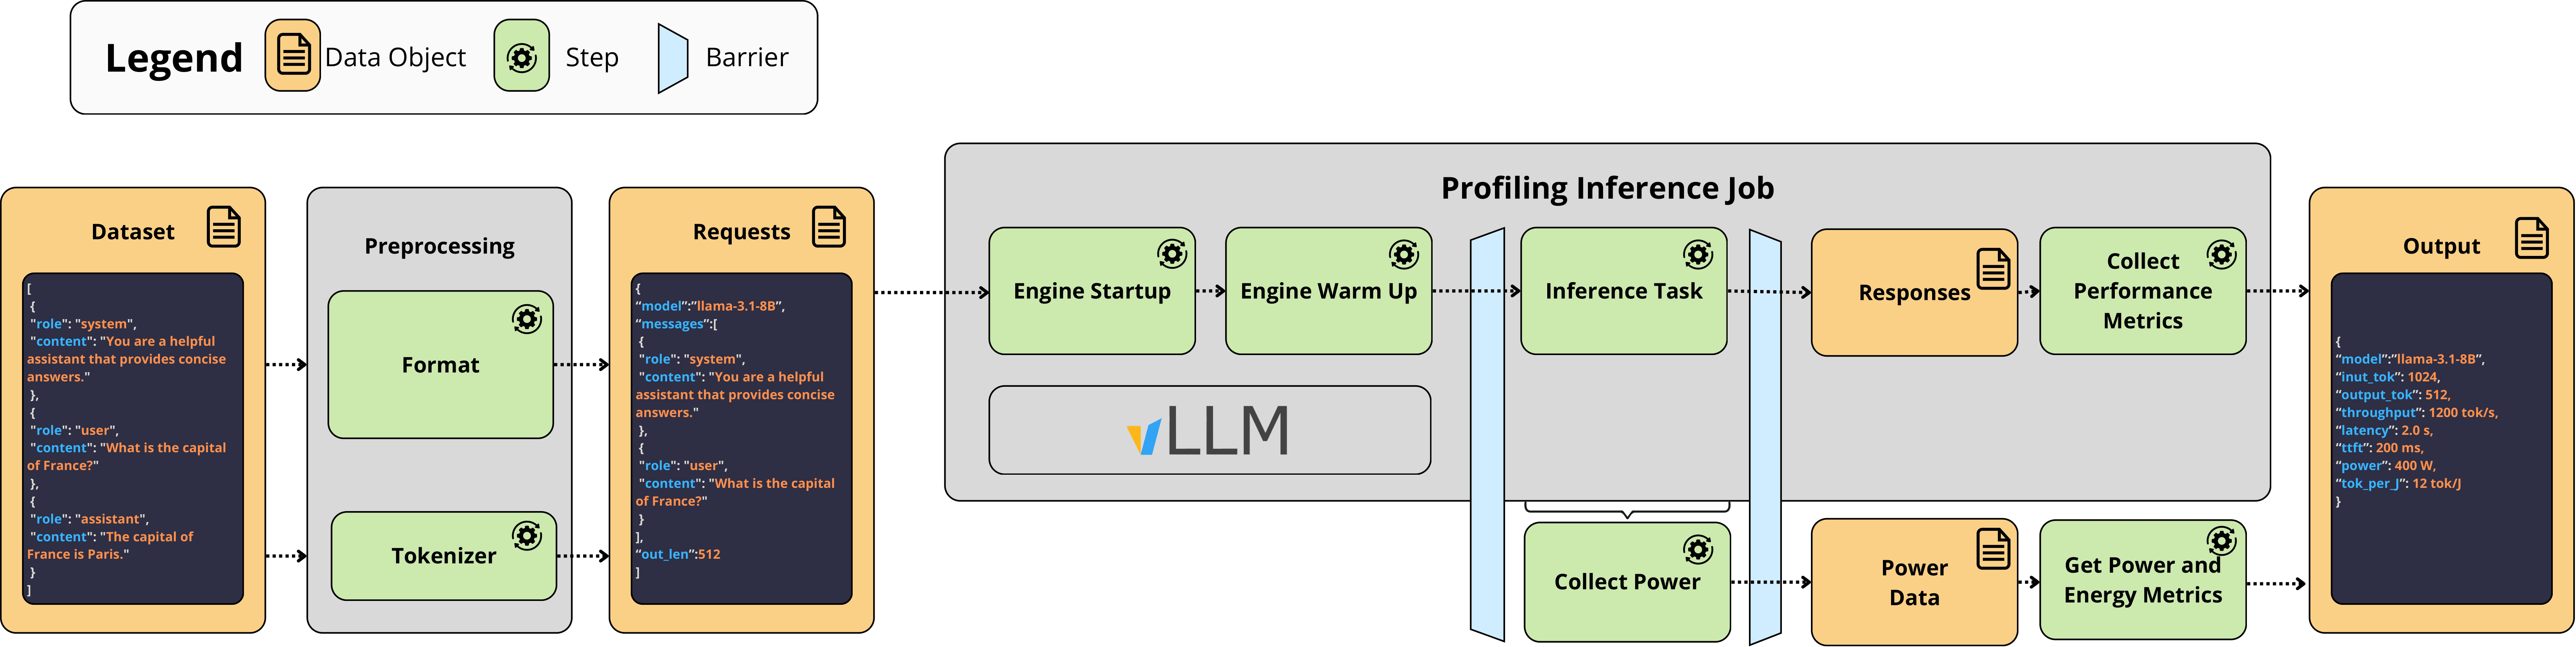
\includegraphics[width=\textwidth]{figs/profile single.png}
    \vspace{5mm}
    \caption{LLM Inference Benchmark Stages.}
    \tagpdfsetup{alttext={LLM Inference Benchmark Stages.}}
    \label{fig:bench}
\end{figure}

To fairly compare those devices, we use a similar software stack on each machine. In particular, we use vLLM \cite{kwon2023efficient}, a high-performance, open-source LLM inference framework compatible with Nvidia, AMD, and Intel GPUs. vLLM allows to achieve superior performance and energy efficiency \cite{fernandez2025energy} compared to the standard Transformers \cite{wolf2019huggingface} implementation by leveraging some key optimizations like the FlashAttention Backend \cite{dao2022flashattention}, PagedAttention \cite{kwon2023efficient}, and continuous batching \cite{agrawal2023sarathi}.
\ref{tab:nodes} reports the specific software stack used on each machine, including the GPU driver, PyTorch version, and vLLM version.

\begin{table}[h!]
\centering
\footnotesize
\caption{GPU nodes used in the experimental evaluation.}
\label{tab:nodes}

\begin{tabularx}{\textwidth}{l l c c c X}
\toprule
\textbf{Vendor} & \textbf{Name} & \textbf{Precision} & \textbf{GPUs/Node} & \textbf{Driver} & \textbf{Software} \\
\midrule

\textbf{NVIDIA} & \textbf{A100}  & BF16, W8A16 & 8  & CUDA 12.6 & \makecell[l]{Torch 2.7.0 \\ vLLM 0.9.0} \\

\textbf{NVIDIA} & \textbf{H100}  & BF16, W8A8  & 4  & CUDA 12.6 & \makecell[l]{Torch 2.7.0 \\ vLLM 0.9.0} \\

\textbf{NVIDIA} & \textbf{GH200} & BF16, W8A8  & 1  & CUDA 12.9 & \makecell[l]{Torch 2.7.0 \\ vLLM 0.9.0} \\

\midrule

\textbf{AMD} & \textbf{MI250}  & BF16        & 4 & ROCm 5.3 & \makecell[l]{Torch 2.7.0+rocm \\ vLLM 0.9.1} \\

\textbf{AMD} & \textbf{MI300X} & BF16, W8A8  & 8 & ROCm 5.3 & \makecell[l]{Torch 2.7.0+rocm \\ vLLM 0.9.1} \\

\midrule

\textbf{Intel} & \textbf{MAX 1550} & FP16 & 6 & oneAPI 2025.2.0 & \makecell[l]{Torch 2.8.0a0 \\ vLLM 0.10.1.xpu} \\

\bottomrule
\end{tabularx}
\end{table}

Each experiment starts by initializing the vLLM engine and loading the inference dataset.
Once the model is loaded and the inference engine is ready, we create an independence process that probes the vendor system monitoring interfaces (py3nvml for NVIDIA, amdsmi for AMD, and xpu-smi for Intel) at consistent intervals to capture power consumption, memory usage, and GPU utilization. For NVIDIA and AMD devices, we sample every 0.5 seconds. For Intel, we have an average sampling rate of 1.9 seconds, due to the longer response time of xpu-smi.
We created the profiler and submitted the inference dataset as a unique batch job to the engine using the vLLM chat method.
Once vLLM has generated the replies for each entry of the dataset, it returns an output object containing information about the end-to-end latency, time to first token, and input and output length of each sequence. This information allows us to collect all the performance metrics described in Section \ref{chap:methods:sec:metrics}.
The profiler data, on the other hand, is used to collect power and energy consumption. To ensure that the profiler process probes the GPU's SMIs only when the GPU is active, we synchronize it with the main process using Python multiprocessing barriers.

For each GPU, this experiment uses different models, precisions, and batch sizes.

Concerning the models, we us four open-source models with a size that ranges from 8B to 32B parameters. Precisely, Llama 3.1 8B, Qwen3 14B, Mistral Small 3.1 24B, and Qwen3 32B. The architectural details of those models are reported in \ref{tab:models}, in the next section.

To evaluate different precisions, we rely on vLLM dynamic weight quantization, which allows us to perform W8A16 quantization (8-bit weights and 16-bit activations) or W8A8 quantization (8-bit weights and 8-bit activations) \cite{vllm-fp8-docs-v0_5_4}, depending on the hardware architecture.
On NVIDIA H100 and AMD MI300x, which offer in-hardware support for FP8 quantization, we use W8A8 quantization. On Nvidia A100, instead, we employ W8A16. Other devices are not included in those experiments, as they do not support either.
For the 16-bit precision, we use bfloat16 (Brain Float 16) precision on Nvidia and AMD, as it is the default precision of the models. For Intel instead, we convert to FP16; single-key optimizations are not yet supported for bfloat16 precision.
Finally, we repeat each experiment for batch sizes of 16 to 128.